\documentclass[aspectratio=169,11pt]{beamer}

% -------------------------------------------------
% Theme and packages
% -------------------------------------------------
\usetheme{Madrid}
\usecolortheme{default}

\usepackage[utf8]{inputenc}
\usepackage[T1]{fontenc}
\usepackage{lmodern}
\usepackage{booktabs}
\usepackage{amsmath}
\usepackage{listings}
\usepackage{xcolor}
\usepackage{graphicx}
\usepackage{multicol}
\usepackage{graphicx}
\usepackage{hyperref}
\usepackage{booktabs}
\usepackage{pgfpages}


%\pgfpagesuselayout{2 on 1}[a4paper,border shrink=5mm]

% -------------------------------------------------
% R code style
% -------------------------------------------------
\definecolor{rcodebg}{RGB}{248,248,248}
\definecolor{rcodecomment}{RGB}{80,120,80}
\definecolor{rcodekeyword}{RGB}{0,80,160}
\definecolor{rcodefunction}{RGB}{120,50,120}

\lstdefinelanguage{R}{
	keywords={
		library, require, function, if, else, for, while,
		TRUE, FALSE, NULL, NA, NaN, Inf
	},
	otherkeywords={
		<-, <<-, $, ::
	},
	sensitive=true,
	comment=[l]{\#},
	morestring=[b]",
	morestring=[b]'
}

\lstset{
	language=R,
	backgroundcolor=\color{rcodebg},
	basicstyle=\ttfamily\small,
	keywordstyle=\color{rcodekeyword}\bfseries,
	commentstyle=\color{rcodecomment}\itshape,
	stringstyle=\color{rcodefunction},
	showstringspaces=false,
	breaklines=true,
	frame=single,
	rulecolor=\color{gray!30},
	columns=fullflexible
}

% -------------------------------------------------
% Metadata
% -------------------------------------------------
\title{R for Budget Analysis}
\subtitle{Data Analysis, Visualization and Reproducible Scripts}
\author{}
\institute{Finance Division\\Ministry of Finance, Bangladesh}
\date{28 September 2026}

% -------------------------------------------------
% Footer
% -------------------------------------------------
\setbeamertemplate{footline}{
	\leavevmode%
	\hbox{%
		\begin{beamercolorbox}[
			wd=.85\paperwidth,
			ht=2.5ex,
			dp=1ex,
			leftskip=1em
			]{author in head/foot}
			\insertshorttitle
		\end{beamercolorbox}%
		\begin{beamercolorbox}[
			wd=.15\paperwidth,
			ht=2.5ex,
			dp=1ex,
			center
			]{date in head/foot}
			\insertframenumber{} / \inserttotalframenumber
		\end{beamercolorbox}%
	}
}

% -------------------------------------------------
% Document
% -------------------------------------------------
\begin{document}
	
	% -------------------------------------------------
	% Title Frame 1
	% -------------------------------------------------
	\begin{frame}
		\titlepage
	\end{frame}
	
	% -------------------------------------------------
	% Outline Frame 2
	% -------------------------------------------------
	\begin{frame}{Outline}
		
		\tableofcontents
		
	\end{frame}
	
	% =================================================
	\section{Getting Started with R and RStudio}
	% =================================================
	
	\begin{frame}{What is R?}
		
		\begin{itemize}
			\item \textbf{R} is a programming language and software environment
			for statistical computing and graphics.
			
			\item It is widely used for:
			\begin{multicols}{2}	
			\begin{itemize}
				\item Data analysis
				\item Statistics
				\item Econometrics
				\item Data visualization
				\item Machine learning
				\item Reproducible research
			\end{itemize}
			\end{multicols}
			
			\item R is \textcolor{red}{\textbf{free and open source}}.
			
			\item A large ecosystem of packages extends its capabilities.
			
			\item \textcolor{blue} {\textbf{Reproducible and Replicable}}
			
			\item It has \textcolor{red} { state-of-the-art graphics} capabilities.
			
		\end{itemize}
		
	\end{frame}
	
	
	\begin{frame}{Why Learn R?}
		
		\begin{columns}
			
			\column{0.48\textwidth}
			
			\textbf{Advantages}
			
			\begin{itemize}
				\item Free and open source
				\item Powerful statistical tools
				\item Excellent visualization
				\item Reproducible workflows
				\item Large package ecosystem
				\item Automation of repetitive tasks
			\end{itemize}
			
			\column{0.48\textwidth}
			
			\textbf{Common Applications}
			
			\begin{itemize}
				\item Economic analysis
				\item Budget analysis
				\item Survey data
				\item Forecasting
				\item Policy analysis
				\item Academic research
			\end{itemize}
			
		\end{columns}
		
	\end{frame}
	
	
	\begin{frame}{Excel vs R for Budget Analysis}
		
		\begin{block}{Pros of R}
			\begin{itemize}[<+->]
				\item One single R script can be used for all ministry budget analysis
				\item Capacity of Graph Generation and Analytical Report is far better in R
				\item Everything is reproducible from Scripts within seconds
				\item Strong for small and medium datasets
				\item Reproducible word tables can be generated, for which all cell values will be calculated automatically
				\item Future is Data-driven, so one more skill 
			\end{itemize}
		\end{block}
		
		\begin{block}{Challenges}
			\begin{itemize}[<+->]
				\item Learning curve is steeper
				\item Need some coding skills
				\item Everyday the programs/packages are upgraded.
			\end{itemize}
		\end{block}
		
		
		\vspace{0.3cm}
		
	\end{frame}
	
	
	
	\begin{frame}{R vs. RStudio}
		
		\begin{block}{R}
			The programming language and statistical computing environment.
			\newline Installation: \href{https://cran.r-project.org/}
			{\textcolor{blue}{\underline{https://cran.r-project.org}}}
			
		\end{block}
		
		\begin{block}{RStudio}
			An Integrated Development Environment (IDE) that makes working with
			R easier.
			\newline Installation: \href{https://posit.co}
			{\textcolor{blue}{\underline{https://posit.co}}}
		\end{block}
		
		\begin{center}
			\begin{tabular}{ll}
				\toprule
				R & Programming language \\
				RStudio & Development environment \\
				R Packages & Additional functionality \\
				Quarto / R Markdown & Reproducible reports \\
				\bottomrule
			\end{tabular}
		\end{center}
		
	\end{frame}
	
	
	
	\begin{frame}
		\centering
		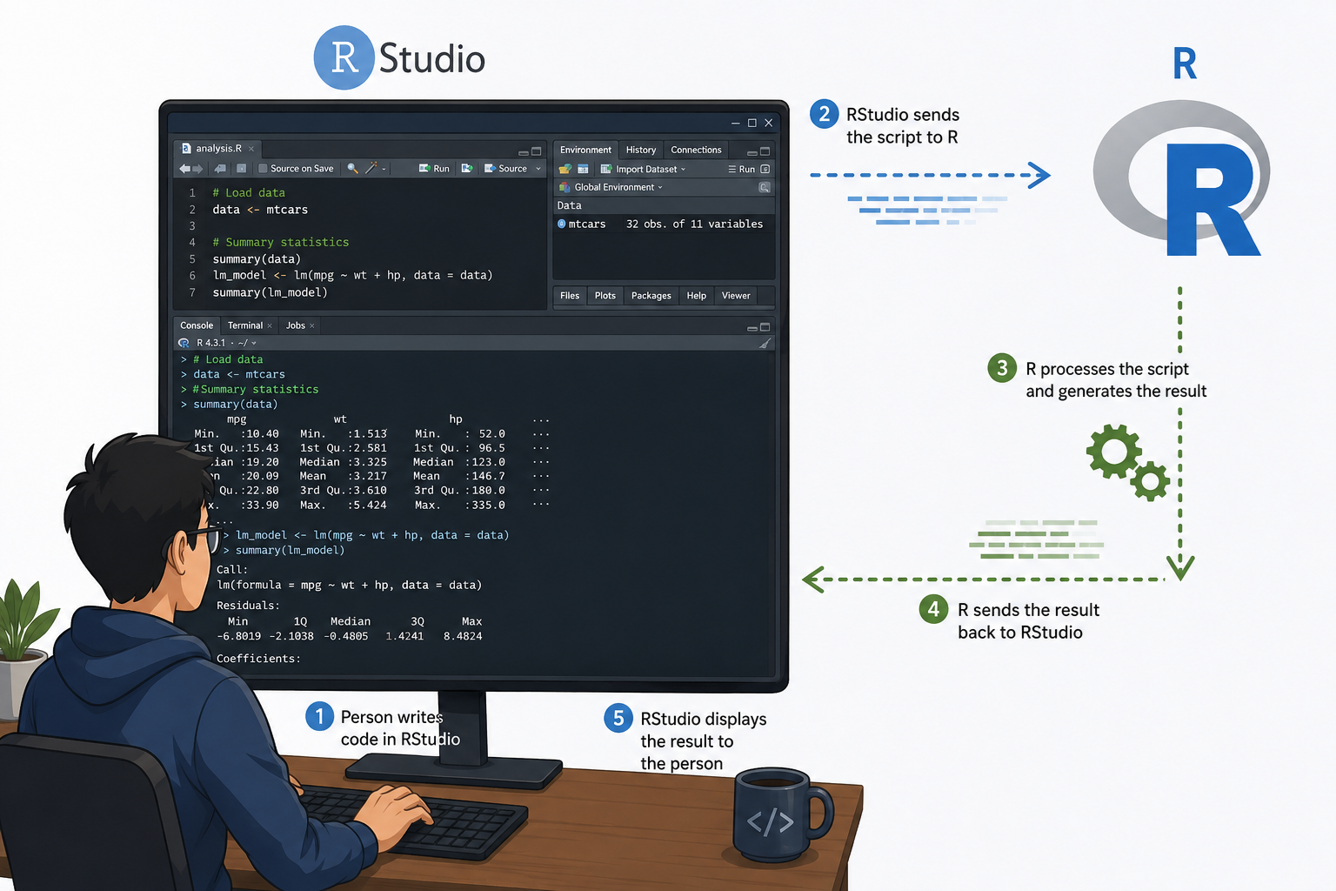
\includegraphics[height=\textheight]{resource/r_rstudio.png}
	\end{frame}
	
	
	\begin{frame}{The RStudio Interface}
		
		Typical RStudio has four major areas:
		
		\begin{enumerate}
			\item \textbf{Source Editor} -- write and save R scripts
			\item \textbf{Console} -- execute R commands
			\item \textbf{Environment} -- inspect objects
			\item \textbf{Files / Plots / Packages / Help} -- manage outputs
		\end{enumerate}
		
		\vspace{0.5cm}
		
		\begin{alertblock}{Recommended practice}
			Write your analysis in an \texttt{.R} script rather than typing
			everything directly into the Console.
		\end{alertblock}
		
	\end{frame}
	
	
		
	\begin{frame}
		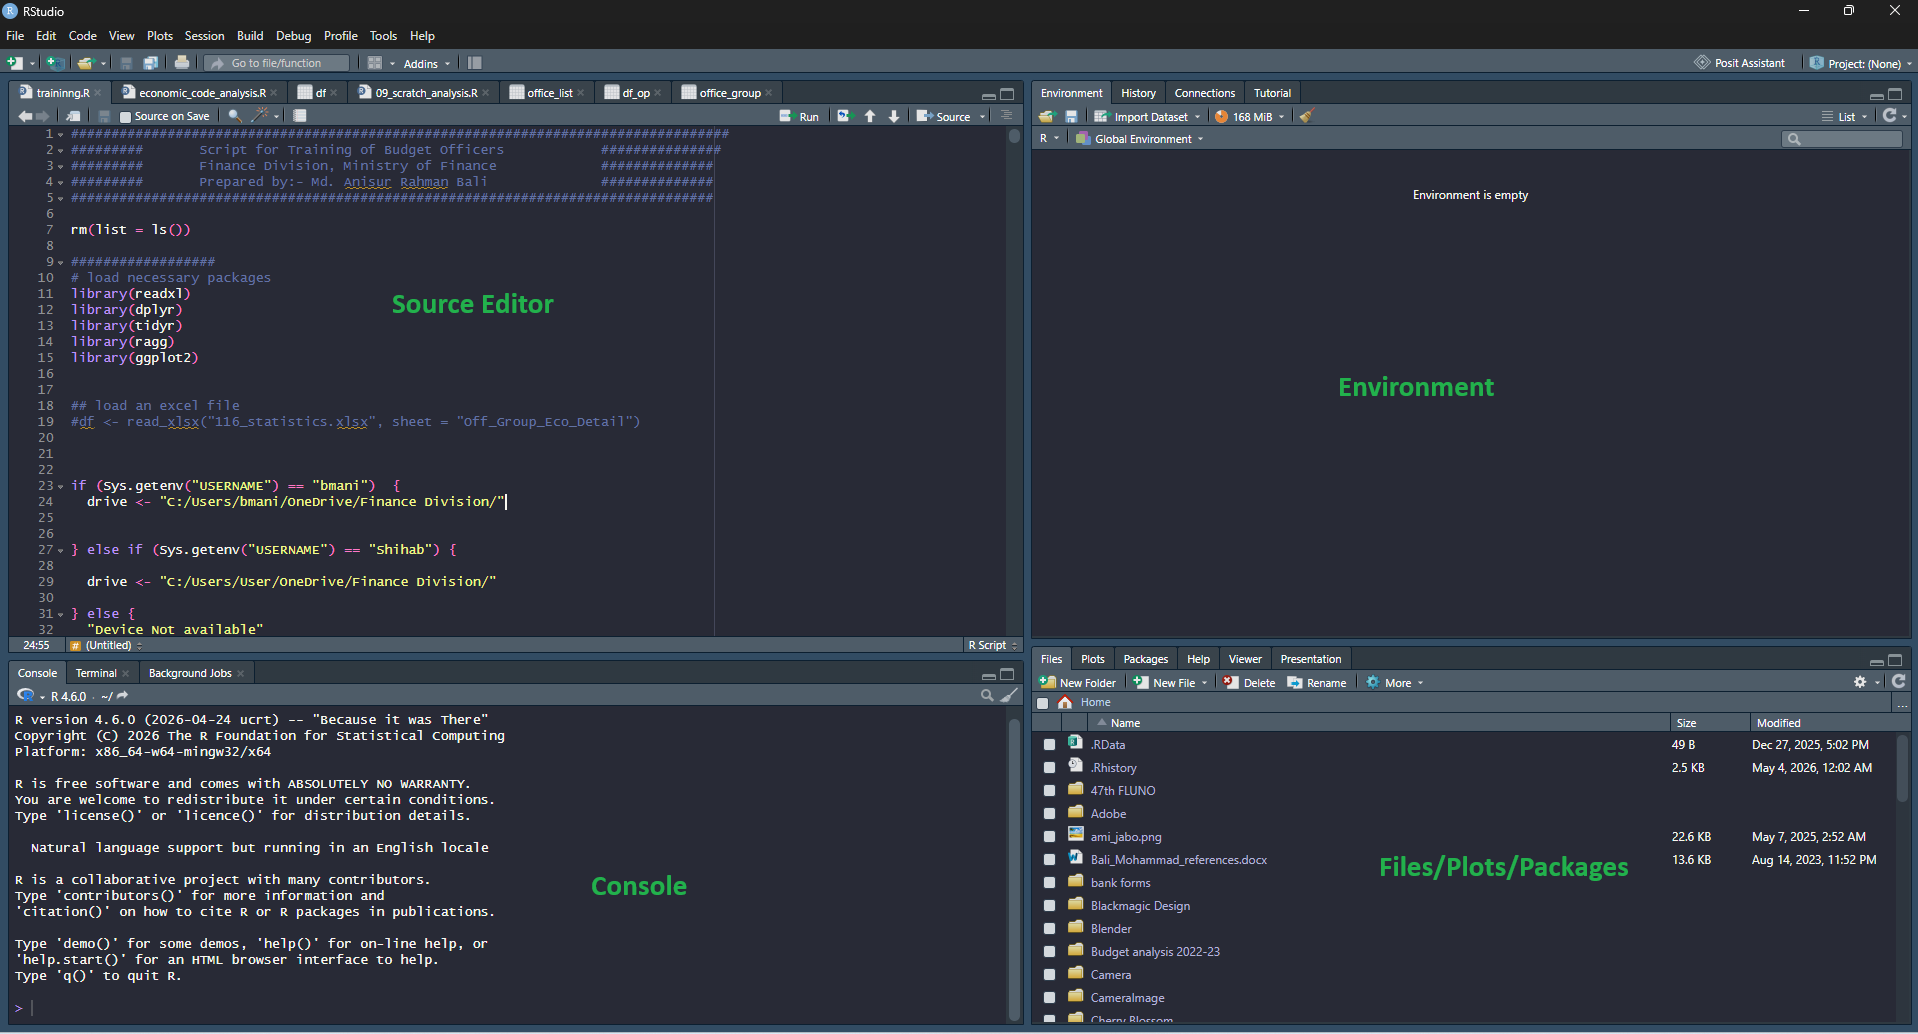
\includegraphics[width=\textwidth]{resource/rstudio_interface.png}
	\end{frame}
	
	
	% =================================================
	\section{Basic R Syntax}
	% =================================================
	
	\begin{frame}[fragile]{Our First R Commands in R Scripts}
		
		Open an R Script and Save it to a folder
		Write the codes in the script		
		\begin{lstlisting}
			2 + 3
			10 * 5
			100 / 4
			2^5
			sqrt(25)
		\end{lstlisting}
		
		To run the a line or few lines, select the lines and click on "Run" or (Ctr + Enter)
		\newline To run the whole script, Click on Source or (Ctr + Shift + Enter)
		\newline To run the previously run block of lines, Clkick Re-run or (Ctr + Alt  P)
		
		\vspace{0.3cm}
	
		
	\end{frame}
	
	
	\begin{frame}[fragile]{Comments in R}
		
		Comments begin with \texttt{\#}.
		
		\begin{lstlisting}
			# Calculate the average expenditure
			
			x <- c(100, 120, 150, 180)
			
			mean(x)
		\end{lstlisting}
		
		Comments are ignored by R.
		
		\vspace{0.4cm}
		
		\begin{block}{Why use comments?}
			Good comments explain \textbf{why} something is being done,
			not merely what the code does.
		\end{block}
		
	\end{frame}
	
	
	\begin{frame}[fragile]{Objects and Assignment}
		
		R stores information in \textbf{objects}, also called \textbf{Variables}.
		
		\begin{lstlisting}
			x <- 100
			name <- "Bangladesh"
			rate <- 0.075
		\end{lstlisting}
		
		The operator \(\boxed{\texttt{<-}}\) is commonly used for assignment.
		\(\boxed{\texttt{=}}\) also works but \(\boxed{\texttt{<-}}\) is preferred
		
		\vspace{0.3cm}
		
		Objects contain data. They can be:
		
		\begin{itemize}
			\item Numbers
			\item Text
			\item Vectors
			\item Data frames
			\item Lists
			\item Functions
		\end{itemize}
		
	\end{frame}
	
	
	\begin{frame}[fragile]{Variable Names}
		
		Good variable names are:
		
		\begin{itemize}
			\item Meaningful
			\item Consistent
			\item Easy to read
		\end{itemize}
		
		\begin{lstlisting}
			total_expenditure <- 150000
			budget_year <- "2025-26"
			ministry_name <- "Ministry of Finance"
		\end{lstlisting}
		
		Avoid:
		
		\begin{lstlisting}
			x1 <- 150000
			a <- "Ministry of Finance"
		\end{lstlisting}
		
		unless the context is obvious.
		
	\end{frame}
	
	
	% =================================================
	\section{Data Types}
	% =================================================
	
	\begin{frame}{Basic Data Types}
		
		Important R data types include:
		
		\begin{table}
			\centering
			\begin{tabular}{ll}
				\toprule
				Type & Example \\
				\midrule
				Numeric & \texttt{123.45} \\
				Integer & \texttt{10L} \\
				Character & \texttt{"Bangladesh"} \\
				Logical & \texttt{TRUE}, \texttt{FALSE} \\
				Factor & Categorical data \\
				Date & \texttt{2026-09-28} \\
				\bottomrule
			\end{tabular}
		\end{table}
		
	\end{frame}
	
	
	
	\begin{frame}[fragile]{Data Structures}
		R provides many built-in data structures. Each is used to handle data in different ways:
		\begin{itemize}
			\item \textbf{Vectors:} A list of items of the same type
			    \begin{lstlisting}[language=R]
				x <- c(10, 20, 30, 40)
			\end{lstlisting}
			\item \textbf{Lists:} can hold different types of data in one structure: numbers, strings, vectors, and even other lists.
			
			 \begin{lstlisting}[language=R]
				thislist <- list("Apple", "Banana", 40, 50)
			\end{lstlisting}
			
			\item \textbf{Matrices:} a 2D data structure where all elements are of the same type.
			\item \textbf{Arrays:} like a matrix but can have more than two dimensions. It stores elements of the same type.
			\item Data Frames
		\end{itemize}
		
	\end{frame}
	
		% =================================================
	\section{Data Frames}
	% =================================================
	
	\begin{frame}[fragile]{Data Structures}
		\textbf{Data Frames:} A data frame is like a table in a spreadsheet. It can hold different types of data across multiple columns. But all values of a column must be similar type. A \textbf{data frame} is one of the most important objects in R.
		
	
	\begin{lstlisting}[language=R]
		df <- data.frame(
				year = c("2023-24", "2024-25", "2025-26"),
				budget = c(100, 120, 150),
				actual = c(95, 110, 130)
				)
		df
	\end{lstlisting}
	
	\vspace{0.2cm}
	
	\textbf{Output:}
	
	\begin{verbatim}
		    	year     	budget    actual
		1     2023-24      	100         95
		2     2024-25      	120        110
		3     2025-26      	150        130
	\end{verbatim}
		
	\end{frame}
	
	
	\begin{frame}[fragile]{Importing Data}
		
		R can work with many formats:
		
		\begin{itemize}
			\item CSV
			\item Excel
			\item Stata
			\item SPSS
			\item SAS
			\item SQL databases
			\item JSON
		\end{itemize}
		
		CSV example:
		
		\begin{lstlisting}
			library(readr)
			df <- read_csv("budget.csv")
		\end{lstlisting}
		
		Excel:
		
		\begin{lstlisting}
			library(readxl)
			df <- read_excel("budget.xlsx")
		\end{lstlisting}
		
	\end{frame}
	
	
	
	\begin{frame}[fragile]{Import a Data Frame and Explore}
		
		Import the exercise.xlsx file:
		
		\begin{lstlisting}[basicstyle=\footnotesize\ttfamily]
			# import the exercise file in the data>raw folder
		
			library(readxl)
			
			read_xlsx("data/raw/exercise.xlsx")
			
			head(df)
			tail(df)
			
			str(df)
			summary(df)
			nrow(df)
			ncol(df)
			names(df)
		\end{lstlisting}
		
		
		These commands help us understand a dataset before analysis.
		
	\end{frame}
	
	
	\begin{frame}{The Dataframe for Exercise}
	
			\centering
			\scriptsize
			
			\begin{columns}[T]
				
				% Operating
				\begin{column}{0.48\textwidth}
					\centering
					\textbf{Operating}
					
					\vspace{0.2cm}
					
					\begin{tabular}{rrrrr}
						\toprule
						Index & year & budget & revised & actual \\
						\midrule
						1  & 2015 & 897  & 843  & 803  \\
						2  & 2016 & 954  & 880  & 863  \\
						3  & 2017 & 1032 & 943  & 911  \\
						4  & 2018 & 1105 & 1104 & 1024 \\
						5  & 2019 & 1176 & 1129 & 1043 \\
						6  & 2020 & 1262 & 1219 & 1074 \\
						7  & 2021 & 1365 & 1205 & 1086 \\
						8  & 2022 & 1406 & 1268 & 1141 \\
						9  & 2023 & 1437 & 1345 & 1336 \\
						10 & 2024 & 1563 & 1417 & 1284 \\
						11 & 2025 & 1613 & 1469 & 1356 \\
						\bottomrule
					\end{tabular}
					
				\end{column}
				
				% Development
				\begin{column}{0.48\textwidth}
					\centering
					\textbf{Development}
					
					\vspace{0.2cm}
					
					\begin{tabular}{rrrrr}
						\toprule
						Index & year & budget & revised & actual \\
						\midrule
						12 & 2015 & 786  & 832  & 677  \\
						13 & 2016 & 934  & 715  & 845  \\
						14 & 2017 & 889  & 919  & 910  \\
						15 & 2018 & 1019 & 905  & 857  \\
						16 & 2019 & 1061 & 1069 & 949  \\
						17 & 2020 & 1252 & 1047 & 1070 \\
						18 & 2021 & 1108 & 1160 & 1050 \\
						19 & 2022 & 1365 & 1208 & 930  \\
						20 & 2023 & 1384 & 1226 & 1085 \\
						21 & 2024 & 1259 & 1321 & 1032 \\
						22 & 2025 & 1379 & 1464 & 1338 \\
						\bottomrule
					\end{tabular}
					
				\end{column}
				
			\end{columns}
		
	\end{frame}
	
	
	
	\begin{frame}[fragile]{R Packages}
		
		\begin{block}{What is an R package?}
			An R package is a collection of functions, datasets, and documentation
			that extends the capabilities of R.
		\end{block}
		
		\vspace{0.3cm}
		\begin{columns}
		\begin{column}{.3\textwidth}
			\textbf{Three basic steps:}
		
		\begin{enumerate}
			\item \textbf{Install} a package
			\item \textbf{Load} the package
			\item \textbf{Use} its functions
		\end{enumerate}
		\end{column}
	
		\begin{column}{.7\textwidth}
	
		\begin{minipage}{0.7\textwidth}
		\begin{lstlisting}[language=R]
	# Install a package (usually done once)
	install.packages("ggplot2")
	
	# Load the package (do this in each new R session)
	library(ggplot2)
	
	# Use a function from the package
	ggplot(data, aes(x = year, y = expenditure)) +
	geom_line()
		\end{lstlisting}
	\end{minipage}
	
		\end{column}	
	\end{columns}
	\end{frame}
	
	
		% =================================================
	\section{Useful R Packages}
	% =================================================
	
	\begin{frame}{Useful Packages for Data Analysis}
		
		\begin{table}
			\centering
			\begin{tabular}{ll}
				\toprule
				Package & Main purpose \\
				\midrule
				\texttt{dplyr} & Data manipulation \\
				\texttt{ggplot2} & Visualization \\
				\texttt{tidyr} & Data reshaping \\
				\texttt{readxl} & Excel files \\
				\texttt{readr} & CSV files \\
				\texttt{data.table} & Fast data processing \\
				\texttt{lubridate} & Dates \\
				\texttt{fixest} & Econometrics \\
				\texttt{modelsummary} & Regression tables \\
				\texttt{sf} & Spatial data \\
				\texttt{quarto} & Reproducible reports \\
				\bottomrule
			\end{tabular}
		\end{table}
		
	\end{frame}
	
	% =================================================
	\section{Tidyverse}
	% =================================================
	
	\begin{frame}[fragile]{The Tidyverse}
		
		\textbf{Tidyverse} is a collection of R packages designed for
		data science.
		
		Important packages include:
		
		\begin{itemize}
			\item \texttt{dplyr} -- data manipulation
			\item \texttt{ggplot2} -- visualization
			\item \texttt{tidyr} -- data reshaping
			\item \texttt{readr} -- importing data
			\item \texttt{stringr} -- text manipulation
			\item \texttt{lubridate} -- dates
		\end{itemize}
		
		Install once: 
		
		\begin{lstlisting}
			install.packages("tidyverse")
		\end{lstlisting}
		
		Load when needed:
		
		\begin{lstlisting}
			library(tidyverse)
		\end{lstlisting}
		
	\end{frame}
	
	
	\begin{frame}[fragile]{Selecting Columns}
		
		We can select a column of Dataframe using \(\boxed{\texttt{\$}}\):
		
		\begin{lstlisting}
			df$budget
			# Make a new df with only one column "budget"
			budget_column <- df$budget
		\end{lstlisting}
		
		Select multiple columns:
		
		\begin{lstlisting}
			df[, c("year", "budget")]
		\end{lstlisting}
		
		Using \texttt{dplyr}:
		
		\begin{lstlisting}
			library(dplyr)
			
			df %>%
			select(year, budget)
		\end{lstlisting}
		
	\end{frame}
	
	
	\begin{frame}[fragile]{The Pipe Operator \& Filtering Rows}
		
		The pipe
		\(
		\boxed{\texttt{\%>\%}}
		\)
		passes the result of one operation to the next.
		
		\begin{lstlisting}
			df %>%
			filter(budget > 1500) %>%
			select(year, budget)
		\end{lstlisting}
		
		Here, \texttt{filter()} keeps only the rows that matches with the condition within () and \texttt{select()} keeps only the columns that matches condition within () 
		\vspace{.5cm}
		\newline
		Newer versions of R also support:
		
		\begin{lstlisting}
			df |>
			filter(budget > 100) |>
			select(year, budget)
		\end{lstlisting}
		
	\end{frame}
	
	
	% =================================================
	\section{Data Manipulation}
	% =================================================
	
	\begin{frame}[fragile]{Logical Expressions}
		
		\begin{center}
			\begin{tabular}{ll}
				\toprule
				Operator & Meaning \\
				\midrule
				\texttt{==} & Equal to \\
				\texttt{!=} & Not equal \\
				\texttt{>} & Greater than \\
				\texttt{>=} & Greater than or equal \\
				\texttt{<} & Less than \\
				\texttt{<=} & Less than or equal \\
				\texttt{\&} & AND \\
				\texttt{|} & OR \\
				\bottomrule
			\end{tabular}
		\end{center}
		
		\begin{lstlisting}
	# condition to select budget is greater than 100
	(budget > 100)
	
	#condition to select budget is greater than 100 and type is operating
	(budget >100 & type == "operating")
		
		\end{lstlisting}
		
		
		
	\end{frame}
	
	
	\begin{frame}[fragile]{Creating Variables with \texttt{mutate()}}
		
		Suppose we want to calculate budget utilization.
		
		\begin{lstlisting}
			df <- df %>%
			mutate(
			utilization = actual / budget
			)
		\end{lstlisting}
		
		Percentage:
		
		\begin{lstlisting}
			df <- df %>%
			mutate(
			utilization_pct = actual / budget * 100
			)
		\end{lstlisting}
		
	\end{frame}
	
	
	\begin{frame}[fragile]{Summarizing Data}
		
		\texttt{summarise()} creates summary statistics.
		
		\begin{lstlisting}[basicstyle=\scriptsize\ttfamily]
		df_summary <- df %>%
			summarise(
			total_budget = sum(budget),
			total_actual = sum(actual),
			average_actual = mean(actual)
			)
		\end{lstlisting}
		
		Grouped summary:
		
		\begin{lstlisting}[basicstyle=\scriptsize\ttfamily]
		df_summary2 <-	df %>%
			group_by(type) %>%
			summarise(
			total_actual = sum(actual)
			)
		\end{lstlisting}
		
		Summarize selected columns by group:
		\begin{lstlisting}[basicstyle=\scriptsize\ttfamily]
		df_summary3 <-	df %>%
			group_by(type) %>%
			summarise(
			across(c(budget, revised, actual), ~mean(.x, na.rm = TRUE)))
		\end{lstlisting}
				
		
		
	\end{frame}
	
	
	\begin{frame}[fragile]{Functions in R}
		
		\begin{block}{What is a function?}
		A function is a name that refers to a reusable piece of code that performs a specific task. Function is written with a parenthesis afterward.
		\end{block}
		
		\vspace{0.3cm}
		
		\begin{columns}[T]
			
			% Built-in functions
			\begin{column}{0.48\textwidth}
				
				\textbf{\large Built-in Functions}
				
				\begin{itemize}
					\item Already available in R
					\item Perform common tasks
					\item Examples:
				\end{itemize}
				
				
				\begin{lstlisting}[language=R]
x <- c(10, 20, 30, 40)

mean(x)
sum(x)
length(x)
max(x)
				\end{lstlisting}
			
				
			\end{column}
			
			% Custom functions
			\begin{column}{0.48\textwidth}
				
				\textbf{\large Custom Functions}
				
				\begin{itemize}
					\item Created by the user
					\item Useful for repeated tasks
				\end{itemize}
				
				\begin{lstlisting}[language=R]
square <- function(x) {
	x^2
}

square(5)
# 25
				\end{lstlisting}
				
			\end{column}
			
		\end{columns}
		
	\end{frame}
	
	
	\begin{frame}[fragile]{Creating a Custom Function}
		
		The basic structure is:
		
		\begin{lstlisting}[language=R]
			function_name <- function(arguments) {
				# code
				return(result)
			}
		\end{lstlisting}
		
		\vspace{0.3cm}
		
		\textbf{Example:}
		
		\begin{lstlisting}[language=R]
			execution_rate <- function(actual, budget) {
				actual / budget * 100
			}
			
			execution_rate(850, 1000)
			# 85
		\end{lstlisting}
		
		\vspace{0.2cm}
		
		\centering
		\textcolor{blue}{Create once $\rightarrow$ Reuse many times}
		
	\end{frame}
	
	\begin{frame}[fragile]{Conditional Statements: \texttt{if}}
		
		\begin{block}{What is an \texttt{if} statement?}
			An \texttt{if} statement executes a block of code only when a specified
			condition is \textbf{TRUE}.
		\end{block}
		
		\vspace{0.3cm}
		
		\textbf{Basic syntax:}
		
		\begin{lstlisting}[language=R]
			if (condition) {
				# code to execute
			}
		\end{lstlisting}
		
		\vspace{0.2cm}
		
		\textbf{Example:}
		
		\begin{lstlisting}[language=R]
			x <- 10
			
			if (x > 5) {
				print("x is greater than 5")
			}
		\end{lstlisting}
		
	\end{frame}
	
	\begin{frame}[fragile]{Conditional Statements: \texttt{if ... else if}}
		
		\vspace{0.3cm}
		
		\textbf{Basic syntax:}
		
		\begin{lstlisting}[language=R]
			if (condition) {
				# code to execute
			} else if (condition){
				# code to execute
			}
		\end{lstlisting}
		
		\vspace{0.2cm}
		
		\textbf{Example:}
		
		\begin{lstlisting}[language=R]
			x <- 10
			
			if (x > 10) {
				print("x is greater than 10")
			} else if (x >5) {
				print("x is less than 15")
			}
		\end{lstlisting}
		
	\end{frame}
	
	\begin{frame}[fragile]{Loops in R: \texttt{for} Loop}
		
		\textbf{A \texttt{for} loop repeats a block of code for each value in a sequence.}
		
		\vspace{0.3cm}
		
		\begin{lstlisting}[basicstyle=\small\ttfamily]
			for (i in 1:5) {
				print(i)
			}
		\end{lstlisting}
		
		\vspace{0.2cm}
		
		\textbf{Example: Loop over budget years}
		
		\begin{lstlisting}[basicstyle=\small\ttfamily]
			years <- 2021:2025
			
			for (year in years) {
				print(year)
			}
		\end{lstlisting}
		
	\end{frame}
	
	\begin{frame}[fragile]{Loops in R: Working with Data Frames}
		
		\textbf{Loop through the rows of a data frame:}
		
		\begin{lstlisting}[basicstyle=\small\ttfamily]
			for (i in 1:nrow(df)) {
				
				row <- df[i, ]
				
				if (row$budget > row$revised) {
					print(row$year)
				}
			}
		\end{lstlisting}
		
		\vspace{0.2cm}
		
		\textbf{Useful control statements}
		
		\begin{itemize}
			\item \texttt{next} -- skip the current iteration
			\item \texttt{break} -- stop the loop completely
		\end{itemize}
		
		
	\end{frame}
	
	
	
	\begin{frame}[fragile]{Exporting Data}
		
		Write a CSV file:
		
		\begin{lstlisting}
			write_csv(df, "data/processed/output.csv")
		\end{lstlisting}
		
		Write an Excel file:
		
		\begin{lstlisting}
			library(writexl)
			write_xlsx(df, "data/processed/output.xlsx")
		\end{lstlisting}
		
		Write the RDS file [R native data]
				\begin{lstlisting}
	
			saveRDS(df, "data/processed/output.rds")
		\end{lstlisting}
		
		\vspace{0.3cm}
		
		\begin{block}{Good practice}
			Keep raw data separate from processed data and analysis outputs.
		\end{block}
		
	\end{frame}
	
	\begin{frame}[fragile]{Converting Data to Long Format}
		
	
		
		\vspace{0.2cm}
		
		\textbf{Convert to long format using \texttt{pivot\_longer()}:}
		
		\begin{lstlisting}[basicstyle=\small\ttfamily]
			df_long <- df %>%
			pivot_longer(
			cols = c(budget, revised, actual),
			names_to = "category",
			values_to = "value"
			)
		\end{lstlisting}
		
		\vspace{0.2cm}
		
		\begin{columns}
			\begin{column}{0.5\textwidth}
				\textbf{Result:}
				
				\textbf{Original data:}
			
			\begin{lstlisting}[basicstyle=\scriptsize\ttfamily]
	year    type        budget  revised  actual
	2015    operating     897      843     803
	2016    operating     954      880     863
	2017    operating    1032      943     911
			\end{lstlisting}
			\end{column}
			
			\begin{column}{0.5\textwidth}
				\textbf{Result:}
				
				\begin{lstlisting}[basicstyle=\scriptsize\ttfamily]
	year       type        category   value
	2015    operating       budget      897
	2015    operating       revised     843
	2015    operating       actual      803
	2016    operating       budget      954
	2016    operating       revised     880
	2016    operating       actual      863
				\end{lstlisting}
				
			\end{column}
		\end{columns}
		
		
	\end{frame}
	
	% =================================================
	\section{Data Visualization}
	% =================================================
	
	\begin{frame}{Data Visualization}
		
		One of the most powerful R visualization packages is:
		\(
		\boxed{\textbf{\texttt{ggplot2}}}
		\)
		\begin{center}
			
		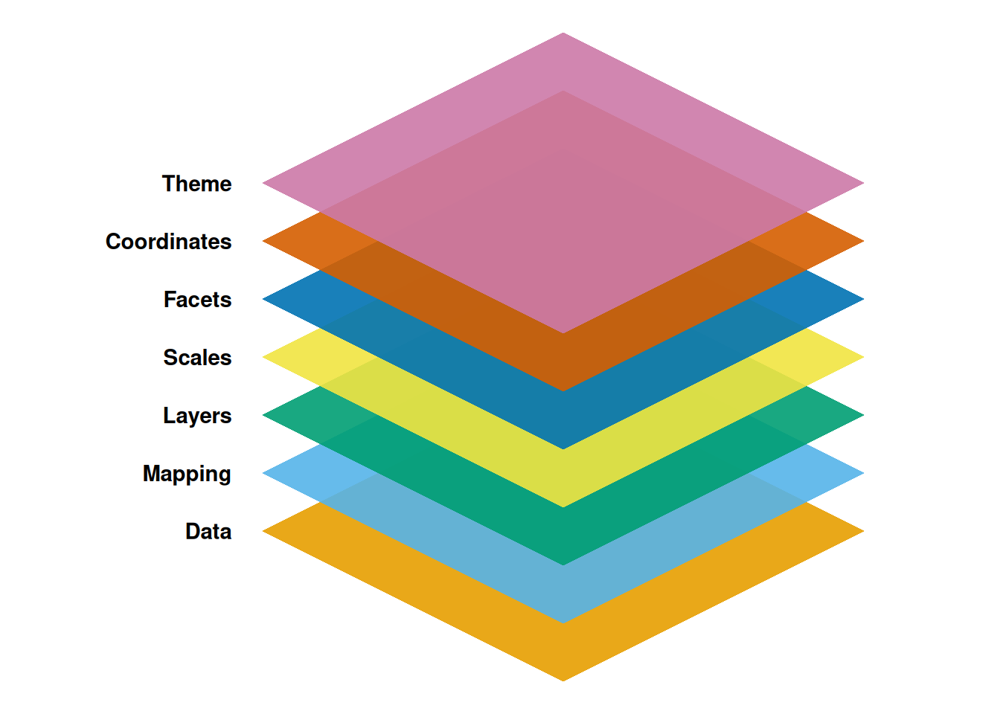
\includegraphics[width=.6\textwidth]{resource/ggplot.png}
	
		\end{center}
	\end{frame}
	
	
	\begin{frame}[fragile]{The Grammar of Graphics}
		
		A \texttt{ggplot2} graph is built from layers.
		
		\begin{lstlisting}
			ggplot(data, aes(x = year, y = actual)) +
			geom_line()
		\end{lstlisting}
		
		Main components:
		
		\begin{enumerate}
			\item Data
			\item Aesthetic mappings
			\item Geometries
			\item Scales
			\item Labels
			\item Themes
		\end{enumerate}
		
	\end{frame}
	
	
	\begin{frame}[fragile]{Bar Chart}
		
		\begin{lstlisting}
			ggplot(df, aes(x = year, y = actual)) +
			geom_col()
		\end{lstlisting}
		
		Grouped bars:
		
		\begin{lstlisting}
			ggplot(df_long,
			aes(x = year,
			y = amount,
			fill = type)) +
			geom_col(
			position = "dodge"
			)
		\end{lstlisting}
		
	\end{frame}
	
	
	\begin{frame}[fragile]{Line Chart}
		
		\begin{lstlisting}
			ggplot(df, aes(x = year,
			y = actual,
			group = 1)) +
			geom_line() +
			geom_point()
		\end{lstlisting}
		
		Useful for:
		
		\begin{itemize}
			\item Time trends
			\item Economic indicators
			\item Budget execution
			\item Inflation
			\item Revenue collection
		\end{itemize}
		
	\end{frame}
	
	
	\begin{frame}[fragile]{Professional Visualization}
		
		A graph can be improved with:
		
		\begin{columns}[T,onlytextwidth]
			
			%------------------------------------------------
			% Left: R code
			%------------------------------------------------
			\begin{column}{0.35\textwidth}
				
				\textbf{R code}
				
				\vspace{0.15cm}
				
				\begin{lstlisting}[
					basicstyle=\tiny\ttfamily,
					frame=single,
					breaklines=true
					]
p <- ggplot(
	df_long,
	aes(
	x = year,
	y = value,
	fill = category
	)
	) +
	
	# Bars
	geom_col(
	position = position_dodge(width = 0.8),
	width = 0.7
	)
				\end{lstlisting}
				
			\end{column}
			
			%------------------------------------------------
			% Right: Graph
			%------------------------------------------------
			\begin{column}{0.65\textwidth}
				
				\centering\textbf{Output}
				
				\vspace{0.15cm}
				
				\centering
				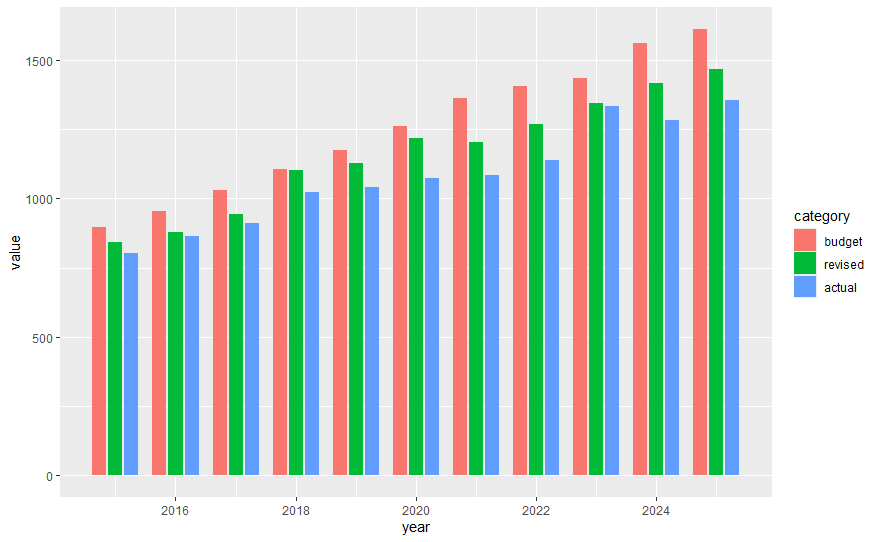
\includegraphics[
				width=\linewidth,
				height=0.70\textheight,
				keepaspectratio
				]{resource/ggplot1.png}
				
			\end{column}
			
		\end{columns}
	\end{frame}
	
	
	\begin{frame}[fragile]{Professional Visualization 2}
		
		A graph can be improved with:
		
		\begin{columns}[T,onlytextwidth]
			
			%------------------------------------------------
			% Left: R code
			%------------------------------------------------
			\begin{column}{0.35\textwidth}
				
				\textbf{R code}
				
				\vspace{0.15cm}
				
				\begin{lstlisting}[
					basicstyle=\tiny\ttfamily,
					frame=single,
					breaklines=true
					]
p +

# Edit the titles of the plot, x and y axis

labs(
	title = "Budget, Actual and Revised Expenditure",
	x = "Fiscal Year",
	y = "Expenditure",
	fill = NULL
) 
				\end{lstlisting}
				
			\end{column}
			
			%------------------------------------------------
			% Right: Graph
			%------------------------------------------------
			\begin{column}{0.65\textwidth}
				
				\centering\textbf{Output}
				
				\vspace{0.15cm}
				
				\centering
				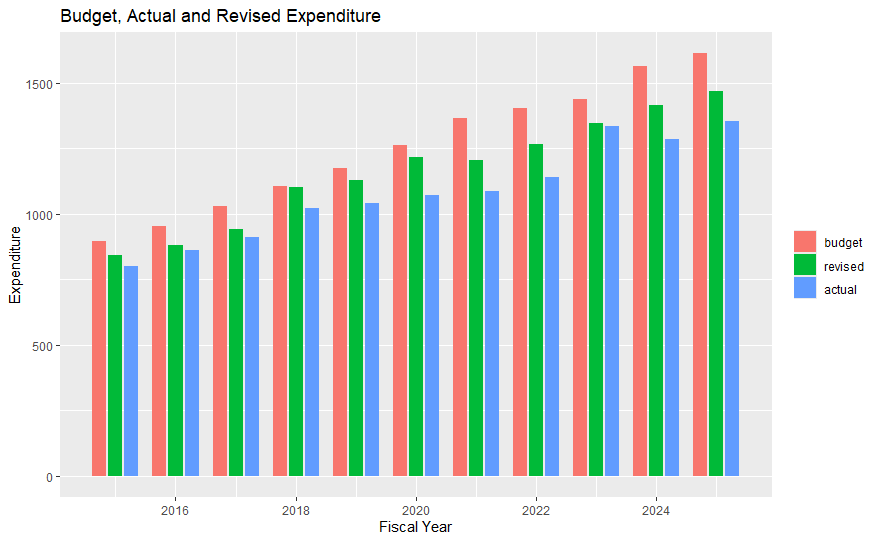
\includegraphics[
				width=\linewidth,
				height=0.70\textheight,
				keepaspectratio
				]{resource/ggplot2.png}
				
			\end{column}
			
		\end{columns}
	\end{frame}
	
	
	\begin{frame}[fragile]{Professional Visualization 3}
		
		A graph can be improved with:
		
		\begin{columns}[T,onlytextwidth]
			
			%------------------------------------------------
			% Left: R code
			%------------------------------------------------
			\begin{column}{0.35\textwidth}
				
				\textbf{R code}
				
				\vspace{0.15cm}
				
				\begin{lstlisting}[
					basicstyle=\tiny\ttfamily,
					frame=single,
					breaklines=true
					]
p +

# edit the bar color and legend label
scale_fill_manual(
	values = c(
		budget = "#4472C4",
		actual = "#70AD47",
		revised = "#ED7D31"
	),
	labels = c(
		budget = "Budget",
		actual = "Actual",
		revised = "Revised"
	)
	) 
				\end{lstlisting}
				
			\end{column}
			
			%------------------------------------------------
			% Right: Graph
			%------------------------------------------------
			\begin{column}{0.65\textwidth}
				
				\centering\textbf{Output}
				
				\vspace{0.15cm}
				
				\centering
				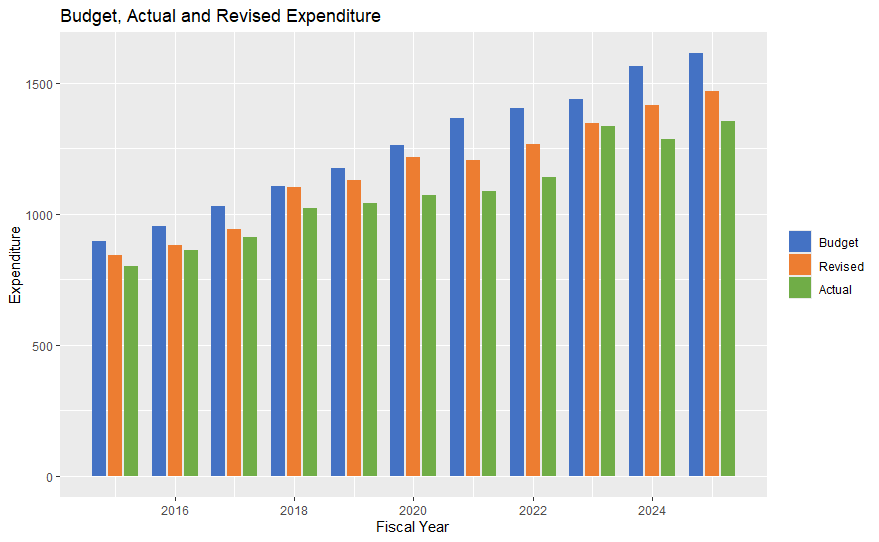
\includegraphics[
				width=\linewidth,
				height=0.70\textheight,
				keepaspectratio
				]{resource/ggplot3.png}
				
			\end{column}
			
		\end{columns}
	\end{frame}
	
	
	\begin{frame}[fragile]{Professional Visualization 4}
		
		A graph can be improved with:
		
		\begin{columns}[T,onlytextwidth]
			
			%------------------------------------------------
			% Left: R code
			%------------------------------------------------
			\begin{column}{0.35\textwidth}
				
				\textbf{R code}
				
				\vspace{0.15cm}
				
				\begin{lstlisting}[
					basicstyle=\tiny\ttfamily,
					frame=single,
					breaklines=true
					]
p +

# edit the y axis values
scale_y_continuous(
	labels = scales::comma,
	expand = expansion(mult = c(0, 0.05))
) +

# x axis to show all the years
scale_x_continuous(
	breaks = 2015:2025,
	labels = 2015:2025
)
				\end{lstlisting}
				
			\end{column}
			
			%------------------------------------------------
			% Right: Graph
			%------------------------------------------------
			\begin{column}{0.65\textwidth}
				
				\centering\textbf{Output}
				
				\vspace{0.15cm}
				
				\centering
				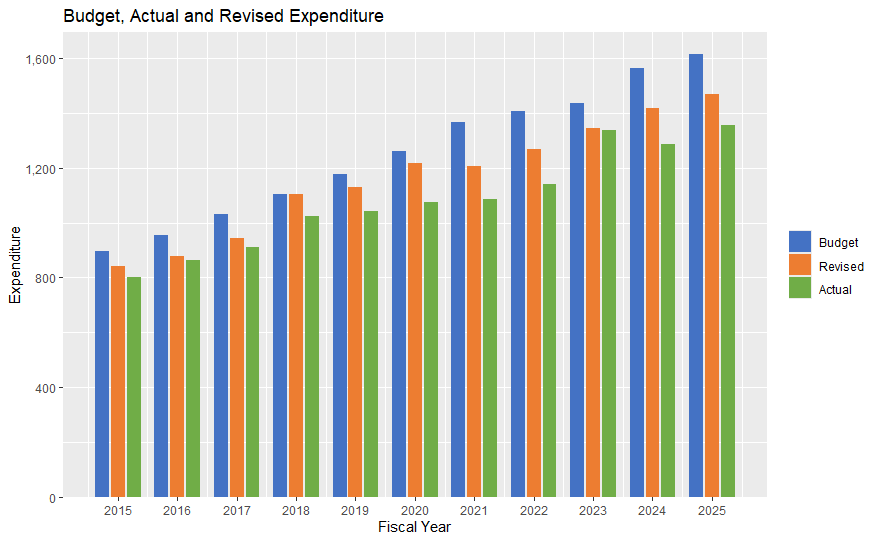
\includegraphics[
				width=\linewidth,
				height=0.70\textheight,
				keepaspectratio
				]{resource/ggplot4.png}
				
			\end{column}
			
		\end{columns}
	\end{frame}
	
	
	\begin{frame}[fragile]{Professional Visualization 5}
		
		A graph can be improved with:
		
		\begin{columns}[T,onlytextwidth]
			
			%------------------------------------------------
			% Left: R code
			%------------------------------------------------
			\begin{column}{0.35\textwidth}
				
				\textbf{R code}
				
				\vspace{0.15cm}
				
				\begin{lstlisting}[
					basicstyle=\tiny\ttfamily,
					frame=single,
					breaklines=true
					]
p +
	
# a theme to use
theme_minimal(base_size = 14)
				\end{lstlisting}
				
			\end{column}
			
			%------------------------------------------------
			% Right: Graph
			%------------------------------------------------
			\begin{column}{0.65\textwidth}
				
				\centering\textbf{Output}
				
				\vspace{0.15cm}
				
				\centering
				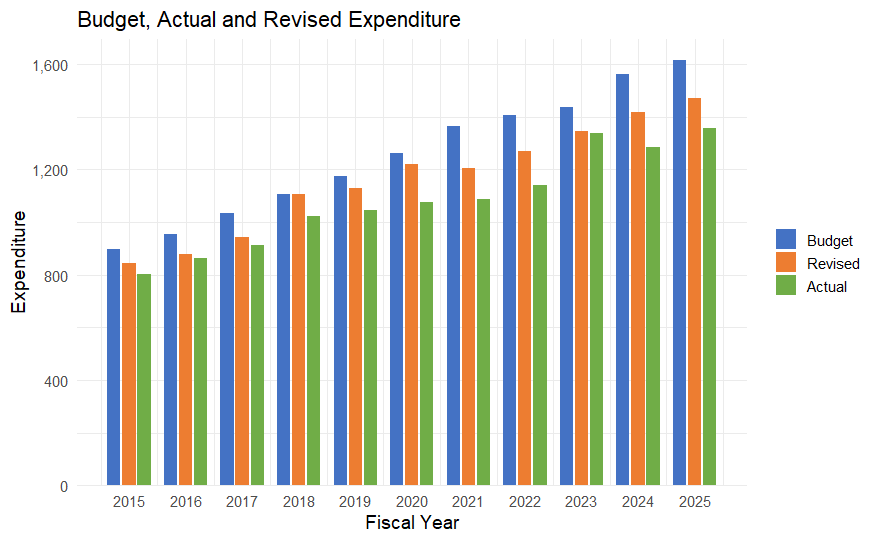
\includegraphics[
				width=\linewidth,
				height=0.70\textheight,
				keepaspectratio
				]{resource/ggplot5.png}
				
			\end{column}
			
		\end{columns}
	\end{frame}
	
	
	\begin{frame}[fragile]{Professional Visualization 6}
		
		A graph can be improved with:
		
		\begin{columns}[T,onlytextwidth]
			
			%------------------------------------------------
			% Left: R code
			%------------------------------------------------
			\begin{column}{0.35\textwidth}
				
				\textbf{R code}
				
				\vspace{0.15cm}
				
				\begin{lstlisting}[
					basicstyle=\tiny\ttfamily,
					frame=single,
					breaklines=true
					]
p +

# editing 
theme(
	plot.title = element_text(
		size = 18,
		face = "bold"
	),
	axis.title = element_text(face = "bold"),
	panel.grid.major.x = element_blank(),
	panel.grid.minor = element_blank(),
	legend.position = "top"
)
					
				\end{lstlisting}
				
			\end{column}
			
			%------------------------------------------------
			% Right: Graph
			%------------------------------------------------
			\begin{column}{0.65\textwidth}
				
				\centering\textbf{Output}
				
				\vspace{0.15cm}
				
				\centering
				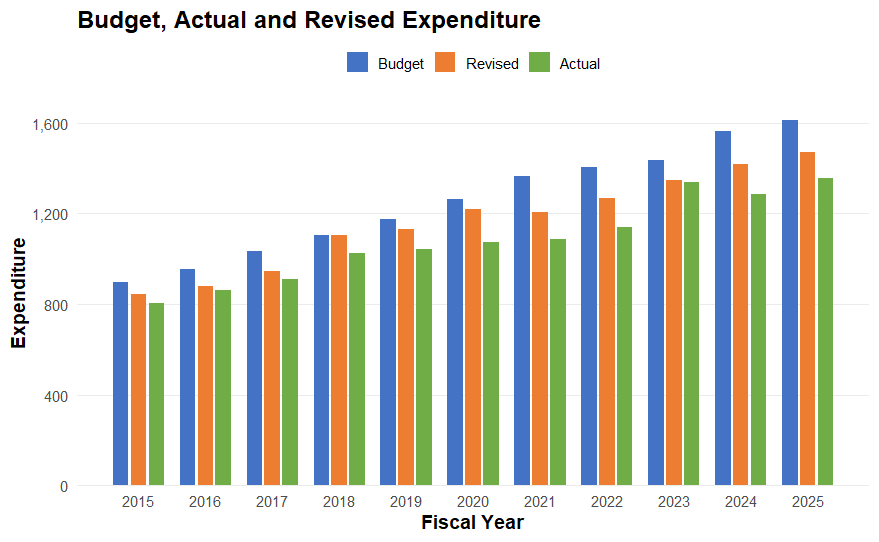
\includegraphics[
				width=\linewidth,
				height=0.70\textheight,
				keepaspectratio
				]{resource/ggplot6.png}
				
			\end{column}
			
		\end{columns}
	\end{frame}
	
	
	% =================================================
	\section{Reproducible Analysis/Research}
	% =================================================
	
	\begin{frame}{Why Reproducibility Matters}
		
		A reproducible analysis allows another person to:
		
		\begin{enumerate}
			\item Obtain the data
			\item Run the code
			\item Reproduce the analysis
			\item Verify the results
		\end{enumerate}
		
		\vspace{0.4cm}
		
		Instead of:
		
		\begin{center}
			\textit{``I calculated this in Excel.''}
		\end{center}
		
		we can provide:
		
		\begin{center}
			\textit{Data + Code + Documentation}
		\end{center}
		
	\end{frame}
	
	
	\begin{frame}[fragile]{A Good R Project Structure}
		
		\begin{lstlisting}[basicstyle=\footnotesize\ttfamily]
			budget-analysis/
			|
			|-- data/
			|   |-- raw/
			|   |-- processed/
			|
			|-- R/
			|   |-- import.R
			|   |-- cleaning.R
			|   |-- analysis.R
			|
			|-- output/
			|   |-- figures/
			|   |-- tables/
			|
			|-- report/
			|
			|-- budget-analysis.Rproj
		\end{lstlisting}
		
	\end{frame}
	
	

	
	
	% =================================================
	\section{Best Practices}
	% =================================================
	
	\begin{frame}{Good Practices in R}
		
		\begin{enumerate}
			\item Use meaningful variable names.
			\item Keep raw data unchanged.
			\item Use scripts instead of relying on the Console.
			\item Comment important decisions.
			\item Use functions for repeated operations.
			\item Keep projects organized.
			\item Use version control when possible.
			\item Make analysis reproducible.
		\end{enumerate}
		
	\end{frame}
	
	
	
	
	\begin{frame}{A Typical R Workflow}
		
		\begin{center}
			
			\large
			Import Data
			
			$\downarrow$
			
			Clean Data
			
			$\downarrow$
			
			Explore Data
			
			$\downarrow$
			
			Transform Data
			
			$\downarrow$
			
			Analyze Data
			
			$\downarrow$
			
			Visualize Results
			
			$\downarrow$
			
			Communicate Findings
			
		\end{center}
		
	\end{frame}
	
	
	
	% =================================================
	\section{Conclusion}
	% =================================================
	
	\begin{frame}{What can be done for Budget Analysis}
		
		\begin{itemize}
			\item Graphs for Working Paper can be automated.
			
			\item Tables for Working Paper can be automated.
			
			\item Economic code wise and office wise graphs can be generated to see the trends
			
			\item Finding out the anomalies.
			
			\item Generating reports
		\end{itemize}
		
	\end{frame}
	
	
	\begin{frame}{Final Message}
		
		\begin{center}
			
			\Huge
			\textbf{Don't just learn R.}
			
			\vspace{0.5cm}
			
			\Huge
			\textbf{Use R to answer questions.}
			
			\vspace{1cm}
			
			\Large
			Data $\rightarrow$ Evidence $\rightarrow$ Insight
			
		\end{center}
		
	\end{frame}
	
	
	\begin{frame}
		\centering
		\Huge
		\textbf{Thank You}
		
		\vspace{0.5cm}
		
		\Large
		Questions?
		
	\end{frame}
	
	\end{document}